\section{Patron de reconfiguration}

%
\begin{frame}{Comparaison des critères de réutilisation des décisions de reconfiguration
pour les SdSs}
\begin{table}[]
\resizebox{\textwidth}{!}{%
\centering
\begin{tabular}{|c|c|c|c|c|c|c|}
\hline
\backslashbox{Auteurs}{Critères}               & Titre     & Intention & Contexte  & Problème  & Solution  & Conséquence \\
\hline
Allen, 1998    & \ding{53} & \ding{53} & Partielle & Partielle & Partielle & \ding{53}   \\
\hline
Oliveira, 2015 & Partielle & \ding{53} & Partielle & Partielle & Partielle & \ding{53}   \\
\hline
Gomaa, 2004    & Partielle & \ding{53} & Partielle & \ding{53} &\ding{51}  & \ding{53}   \\
\hline
\end{tabular}
}
\end{table}
\end{frame}

\begin{frame}{Réutilisation des décisions de reconfiguration}
\begin{columns}
\begin{column}{0.5\textwidth}
\textbf{Titre}\\
Métaphore\\
%\setlength\itemsep{0.7cm}
\vspace{1mm}
\textbf{Intention}\\
Desc. informelle\\
\vspace{1mm}
\textbf{Contexte}\\
Diagr. de block archi.
\begin{itemize}
\item utile à la compréhension d'un problème de reconfiguration
\item adapté à la modélisation de système complexe
\end{itemize}                                                                   
\textbf{Problème}\\
Diagr. de block archi. source et ciblée 
\begin{itemize}
\item description des parties impliquées par la reconf. 
\end{itemize}
\end{column}
\begin{column}{0.5\textwidth}
Desc. informelle invariants
\begin{itemize}
\item difficultés à résoudre
\end{itemize}             
Desc. informelle forces                                                         
\begin{itemize}
\item principe de la solution
\end{itemize}             
\textbf{Solution}\\
Diagr. état + descript. informelle                                                              
\begin{itemize}
\item états du médiateur de reconf.
\item opérations à implémenter
\item événements de reconf.
\end{itemize}             
\textbf{Conséquence}\\
Descr. informelle
\begin{itemize}
\item discutions et propositions sur choix d'implementation 
\end{itemize}             
\end{column}
\end{columns}
\end{frame}

\begin{frame}{Patron de reconfiguration : co-évolution}
\centering
\flushleft
Titre : Co-évolution\\
Intention : \\
\begin{figure}
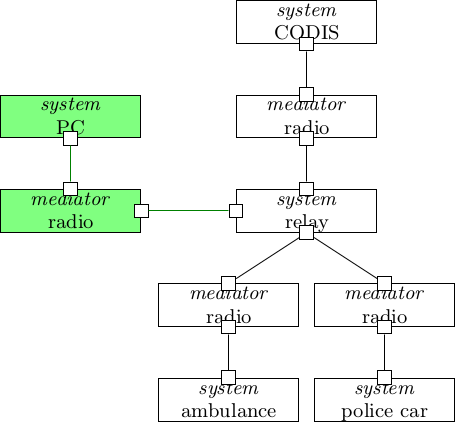
\includegraphics[height=2.5cm]{imgs/fig_rearchitecture}
\caption{\underline{\textbf{Exemple service des secours}}}
\end{figure}
\end{frame}

\begin{frame}{Patron de reconfiguration co-évolution : délimitation du problème}
\begin{figure}
\begin{subfigure}[b]{0.4\textwidth}
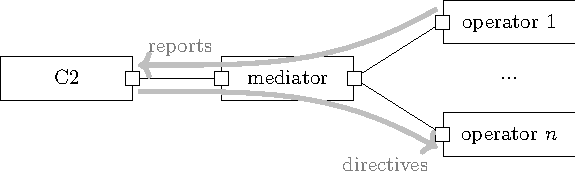
\includegraphics[width=4cm]{imgs/dc-context}
\caption{Contexte}
\end{subfigure}
\begin{subfigure}[b]{0.4\textwidth}
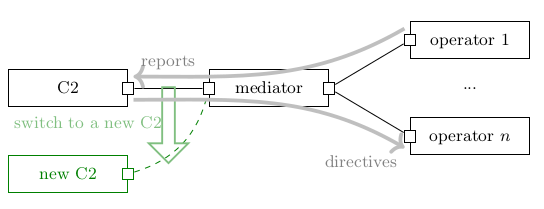
\includegraphics[width=4cm]{imgs/dc_archi-C2}
\caption{Problématique}
\end{subfigure}
\end{figure}

Invariants :
\begin{itemize}
\item Les deux C2 partagent le même état de mission.
\item Tous les opérateurs sont connectés à exactement un
C2. 
\end{itemize}

Forces :
\begin{itemize}
\item Instancier une deuxième version du composant qui coexiste avec
la version initiale.
\item Synchroniser les états partagés entre les versions du
composant.
\end{itemize}

\end{frame}

\begin{frame}{Patron de reconfiguration : description de la solution}
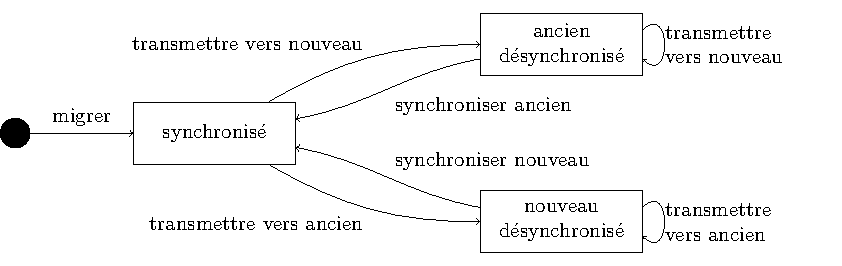
\includegraphics[width=12cm]{imgs/slide_solution_coevolution.pdf}
\end{frame}


\begin{frame}{Patrons de reconfiguration supplémentaires}
\begin{itemize}
\setlength\itemsep{0.7cm}
\item \underline{\textbf{Quiescence}} : rendre passif,
les composants dépendant du composant ciblé par la reconfiguration. 
\item \underline{\textbf{Tranquilité}} : variante de la quiescence qui assouplie
les critères de reconfiguration. Elle décrit les conditions dans
lesquelles la reconfiguration peut-être réalisée sans attendre l'état de
quiescence
\item \underline{\textbf{Co-evolution}} : déployer directement la nouvelle version du composant ciblé par la
reconfiguration. Les deux versions d'un
composant s'executent simultanément. 
\item \underline{\textbf{Opportuniste}} : une opération de
déconnexion et connexion qui est réalisée dès que l'occasion se
présente.  
\end{itemize}
\end{frame}
